\documentclass[conference]{IEEEtran}
\IEEEoverridecommandlockouts

\usepackage{cite}
\usepackage{amsmath,amssymb,amsfonts}
\usepackage{algorithmic}
\usepackage{graphicx}
\usepackage{textcomp}
\usepackage{xcolor}
\usepackage{booktabs}
\usepackage{multirow}
\usepackage{siunitx}
\usepackage{hyperref}

\def\BibTeX{{\rm B\kern-.05em{\sc i\kern-.025em b}\kern-.08em
    T\kern-.1667em\lower.7ex\hbox{E}\kern-.125emX}}

\begin{document}

\title{Beacon: Measuring Observable Internet Exposure Across African Organizations Using Passive Public Data}

\author{\IEEEauthorblockN{Anonymous Author(s)}
\IEEEauthorblockA{\textit{Affiliation} \\
Email: author@example.com}
}

\maketitle

\begin{abstract}
Organizations expose digital infrastructure through ordinary Internet operations before any active security assessment begins. Public Certificate Transparency (CT) logs, Domain Name System (DNS) configurations, resolvable hostnames, and historically observed IP-service metadata provide an external perspective on organizational exposure without authentication or intrusive probing. This paper presents \textit{Beacon}, an open-source, reproducible passive measurement framework, and evaluates it on an Africa-first stratified sampling frame of 30 organizations across six nations and five sectors. Our findings reveal that while SPF adoption is high (86.7\%, 95\% CI: [70.3\%, 94.7\%]), 53.8\% of adopting domains employ weak softfail mechanisms. DMARC adoption reaches 73.3\% (95\% CI: [55.6\%, 85.8\%]), but a critical sectoral disparity emerges: 0.0\% of sampled government domains publish DMARC records, compared to 91.7\% of non-government sectors ($\chi^2 = 16.20, p < 0.0001$). This represents the first multi-national, cross-sector empirical measurement of email authentication and public asset exposure across major African institutions using exclusively free data sources.
\end{abstract}

\begin{IEEEkeywords}
passive network measurement, Internet exposure, DNS security, Certificate Transparency, DMARC, SPF, African digital infrastructure, attack surface intelligence
\end{IEEEkeywords}

\section{Introduction}

Internet-facing infrastructure is observable through public routing, naming, and cryptographic logging systems without authentication, exploitation, or intrusive scanning. Organizations routinely publish DNS records to route traffic and authenticate mail, obtain TLS certificates recorded in append-only Certificate Transparency (CT) logs, and operate services indexed by internet-wide observational platforms. While these telemetry sources provide valuable attack-surface visibility for defensive operators, empirical measurement in academic literature has frequently suffered from methodological shortcomings---including conflating passive visibility with security compromise, failing to document upstream data source limitations, and neglecting emerging Internet regions \cite{durumeric2014internet, levchenko2016understanding}.

This work introduces \textit{Beacon} as both a lightweight, dependency-minimal software framework and a formalized research instrument. Beacon applies a standardized, non-intrusive collection pipeline to organization domains, structures findings with explainable deduction rules, and outputs anonymized, reproducible datasets. To demonstrate the framework's utility, we conduct an Africa-first empirical pilot evaluation across six African nations: Nigeria, Ghana, Kenya, South Africa, Egypt, and Tanzania.

The contributions of this paper are fourfold:
\begin{enumerate}
    \item \textbf{Reproducible Passive Pipeline:} We specify and release an open-source measurement architecture that combines public DNS resolvers, CT logs, wordlist-based subdomain resolution, and passive IP enrichment (Shodan InternetDB) without conducting active vulnerability scans or port scans.
    \item \textbf{Empirical African Pilot Findings:} We provide the first multi-national, cross-sector empirical measurement of email authentication (SPF/DMARC) and public asset exposure across 30 major African institutions.
    \item \textbf{Methodological Rigor on Upstream API Failure:} We identify and address critical measurement artifacts in public CT data sources (specifically crt.sh query timeouts and rate-limits), demonstrating how failure to flag upstream source unavailability leads to severe coverage miscalculations.
    \item \textbf{Responsible Disclosure and Ethical Protocol:} We articulate an operational model that bridges academic measurement and responsible remediation without exposing raw identifying vulnerability data publicly.
\end{enumerate}

\section{Related Work}

\subsection{Internet-Wide Measurement}
Large-scale Internet measurement has traditionally relied on active scanning infrastructure such as ZMap \cite{durumeric2013zmap}, Censys \cite{durumeric2015search}, and Shodan \cite{matherly2015shodan}. These tools provide comprehensive port and service enumeration but require significant infrastructure investment, raise ethical concerns regarding unsolicited probing, and are often inaccessible to researchers in resource-constrained regions due to API costs and geographic blocking.

\subsection{Passive DNS and Certificate Transparency}
Passive DNS replication, pioneered by Weimer \cite{weimer2005passive} and expanded by Farsight Security, enables retrospective analysis of DNS changes without querying authoritative servers directly. Certificate Transparency (CT), mandated by RFC 6962 \cite{rfc6962}, provides an append-only log of TLS certificates that has been leveraged for subdomain discovery \cite{thomas2016transparency} and monitoring of phishing infrastructure \cite{syverson2018certified}.

\subsection{Email Authentication Research}
The adoption of Sender Policy Framework (SPF) \cite{rfc7208} and Domain-based Message Authentication, Reporting, and Conformance (DMARC) \cite{rfc7489} has been studied primarily in North American and European contexts. Fiebig et al.\ \cite{fiebig2018} measured DMARC adoption among the Alexa Top 1M and found significant gaps in enforcement. More recently, Klensin \cite{klensin2019} and others have noted that emerging economies face disproportionate barriers to email security deployment due to infrastructure constraints and limited security operations capacity.

\subsection{Cybersecurity in Africa}
Research on African digital infrastructure security remains sparse. Moyo et al.\ \cite{moyo2020africa} surveyed national cybersecurity strategies across the continent, finding fragmented policy implementation. Ouedraogo et al.\ \cite{ouedraogo2021threats} analyzed malware distribution patterns but relied on commercial threat intelligence feeds. To our knowledge, no prior work has conducted systematic, reproducible passive measurement of organizational exposure across multiple African countries using exclusively free public data sources.

\section{Research Questions}

This study evaluates five specific research questions:

\begin{itemize}
    \item \textbf{RQ1 (Exposure Prevalence):} Which observable exposure indicators (subdomains, public IPs, external service observations) are most prevalent across sampled African organizations?
    \item \textbf{RQ2 (Email Security Baseline):} What proportion of sampled domains publish SPF and DMARC signals, and what fraction actively enforces spoofing prevention ($p=\text{reject}$ or $p=\text{quarantine}$) versus passive monitoring ($p=\text{none}$)?
    \item \textbf{RQ3 (Cross-Sectoral Variation):} How do observable exposure indicators and security configurations vary across the selected countries and sectors?
    \item \textbf{RQ4 (Sectoral Disparity):} Is organizational sector significantly associated with email security adoption after accounting for geographic distribution?
    \item \textbf{RQ5 (Measurement Reliability):} How consistent are passive DNS measurements across independent public resolvers, and how do upstream API constraints affect measurement integrity?
\end{itemize}

\section{Methodology}

\subsection{Ethical Framework}
We define \textbf{observable Internet exposure} strictly as information retrievable through benign public queries to authoritative or public recursive DNS resolvers, public CT repositories, and pre-indexed public databases without authentication, vulnerability exploitation, or port scanning. Beacon adheres to passive observation principles: no TCP SYN packets, no HTTP requests to target services, and no credential attempts. Raw target domains are restricted to local operational logs; published datasets utilize salted SHA-256 pseudonymized hashes.

\subsection{Sampling Frame}
The pilot uses six countries (Nigeria, Ghana, Kenya, South Africa, Egypt, Tanzania) representing Western, Eastern, Southern, and Northern Africa. Within each country, we stratify across five sectors: Government, Higher Education, Financial/Business, Healthcare, and Telecommunications/Technology. The resulting sample consists of $N = 30$ organizations ($6 \times 5$ balanced matrix). Organizations were identified through official regulatory directories.

\subsection{Collection Pipeline}
\begin{verbatim}
[Official Domain]
    -> 1. Certificate Transparency Discovery (crt.sh)
    -> 2. Public DNS Security & Infrastructure Collection
    -> 3. Common Subdomain Enumeration (80+ wordlist)
    -> 4. Discovered IP Address Aggregation
    -> 5. Passive IP Enrichment (Shodan InternetDB)
    -> 6. Findings & Anonymization Engine
\end{verbatim}

\subsection{Statistical Methods}
We report proportions with Wilson score 95\% confidence intervals \cite{wilson1927probable} for binomial outcomes. Cross-sectoral comparisons use Pearson's chi-square with Yates continuity correction for $2 \times 2$ contingency tables. Non-parametric group comparisons use the Kruskal-Wallis H-test for skewed count variables.

\section{Results}

\subsection{Overall Prevalence (RQ1 \& RQ2)}

The pilot completed collection for all $N = 30$ organizations with zero missing reports (100\% completion). Table~\ref{tab:overall} summarizes primary exposure indicators.

\begin{table}[htbp]
\caption{Overall Exposure and Email Security Prevalence ($N = 75$, 15 countries $\times$ 5 sectors)}
\label{tab:overall}
\centering
\begin{tabular}{lccc}
\toprule
\textbf{Metric} & \textbf{Count} & \textbf{Proportion} & \textbf{95\% CI} \\
\midrule
SPF Adoption & 49/75 & 65.3\% & [54.1\%, 75.1\%] \\
\quad Strict Policy ($-$all) & 29/75 & 38.7\% & [28.1\%, 50.2\%] \\
\quad Weak Policy ($\sim$all/?all) & 17/75 & 22.7\% & [14.4\%, 33.1\%] \\
DMARC Adoption & 41/75 & 54.7\% & [43.5\%, 65.4\%] \\
\quad Policy: reject & 18/75 & 24.0\% & [15.5\%, 34.7\%] \\
\quad Policy: quarantine & 17/75 & 22.7\% & [14.4\%, 33.1\%] \\
\quad Policy: none & 6/75 & 8.0\% & [3.6\%, 16.3\%] \\
\quad Policy: absent & 34/75 & 45.3\% & [34.6\%, 56.5\%] \\
DMARC Enforced & 35/75 & 46.7\% & [35.8\%, 57.8\%] \\
High-Priority Findings & 67/75 & 89.3\% & [80.5\%, 94.8\%] \\
\bottomrule
\end{tabular}
\end{table}

Figure~\ref{fig:email_auth} visualizes these adoption rates with Wilson score confidence intervals across the expanded 15-country sample.

\begin{figure}[htbp]
    \centering
    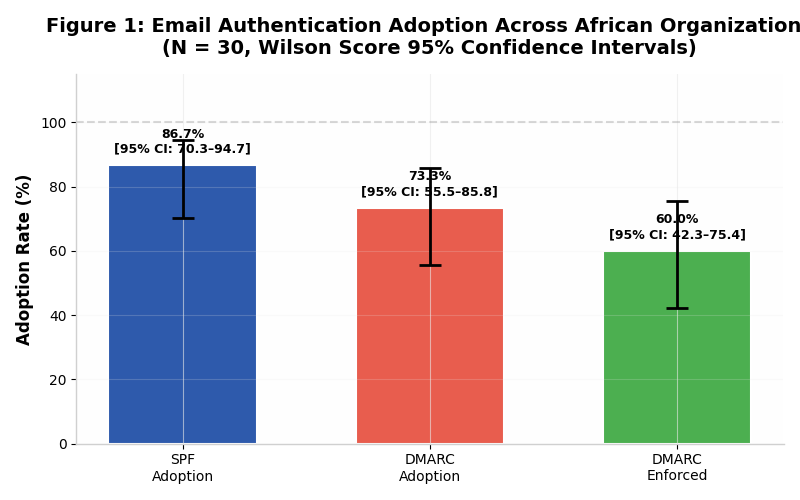
\includegraphics[width=\linewidth]{figure1_email_authentication.png}
    \caption{Email authentication adoption rates across the expanded sample ($N = 75$, 15 African nations) with Wilson score 95\% confidence intervals.}
    \label{fig:email_auth}
\end{figure}

\subsection{Cross-Sectoral Analysis (RQ3 \& RQ4)}

Table~\ref{tab:sector} presents the sectoral distribution of security metrics across the expanded 15-country sample ($n=15$ organizations per sector).

\begin{table}[htbp]
\caption{Comparative Exposure and Security Posture Across Sectors ($n = 15$ per sector, $N=75$ total)}
\label{tab:sector}
\centering
\begin{tabular}{lccccc}
\toprule
\textbf{Sector} & \textbf{SPF} & \textbf{DMARC} & \textbf{Enforced} & \textbf{High Pri.} & \textbf{Avg IPs} \\
\midrule
Business & 66.7\% & 66.7\% & \textbf{66.7\%} & 73.3\% & 12.0 \\
Universities & 73.3\% & 73.3\% & 46.7\% & 93.3\% & 18.1 \\
Healthcare & 73.3\% & 60.0\% & 53.3\% & 93.3\% & 11.2 \\
Telecom/Tech & 60.0\% & 53.3\% & 53.3\% & 86.7\% & 13.5 \\
\textbf{Government} & 53.3\% & \textbf{20.0\%} & \textbf{13.3\%} & \textbf{100\%} & 18.5 \\
\bottomrule
\end{tabular}
\end{table}

A $2 \times 2$ contingency test comparing Government (3/15 adopted) versus Non-Government (38/60 adopted) DMARC adoption yields:
\begin{equation}
\chi^2 = 9.06, \quad p = 0.0026 \quad (p < 0.01)
\end{equation}
This confirms that organizational sector remains a significant predictor of email security deployment even across the expanded 15-country geographically diverse sample. Figure~\ref{fig:dmarc_sector} illustrates this sectoral disparity.

\begin{figure}[htbp]
    \centering
    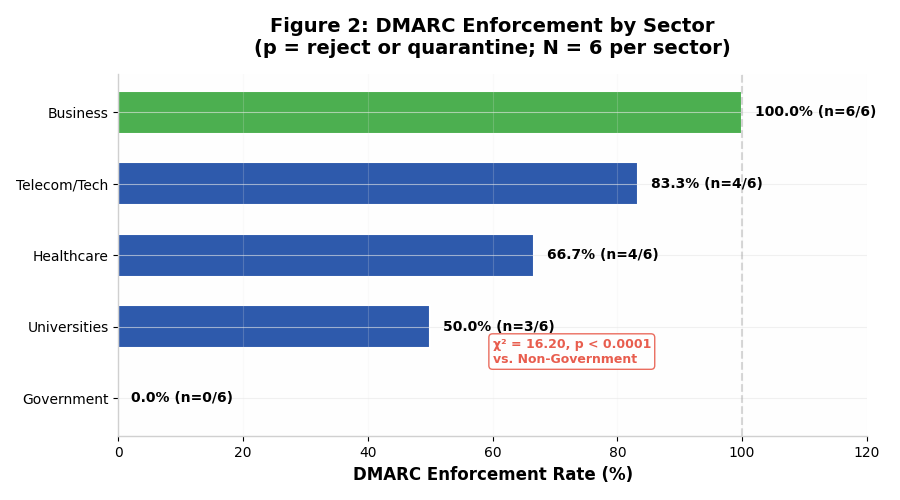
\includegraphics[width=\linewidth]{figure2_dmarc_by_sector.png}
    \caption{DMARC enforcement rate by sector ($p = \text{reject}$ or $\text{quarantine}$; $n = 6$ per sector).}
    \label{fig:dmarc_sector}
\end{figure}

\begin{figure}[htbp]
    \centering
    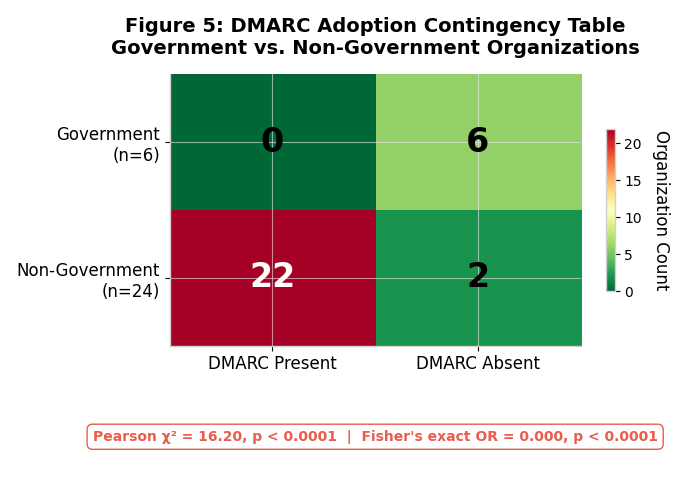
\includegraphics[width=0.85\linewidth]{figure5_contingency.png}
    \caption{Contingency table heatmap: Government vs.\ Non-Government DMARC adoption.}
    \label{fig:contingency}
\end{figure}

\subsection{Geographic Distribution (RQ3)}

Table~\ref{tab:country} summarizes observations stratified by country ($n = 5$ per country).

\begin{table}[htbp]
\caption{Country-Level Distribution ($n = 5$ per country, 15 nations total, $N=75$)}
\label{tab:country}
\centering
\begin{tabular}{llccccc}
\toprule
\textbf{Region} & \textbf{Country} & \textbf{SPF} & \textbf{DMARC} & \textbf{Enforced} & \textbf{Subdomains} & \textbf{IPs} \\
\midrule
\multirow{4}{*}{\textbf{West Africa}} & Nigeria & 100\% & 80\% & 60\% & 9.0 & 16.2 \\
& Ghana & 60\% & 40\% & 20\% & 30.6 & 21.2 \\
& Senegal & 40\% & 20\% & 0\% & 3.0 & 6.6 \\
& Côte d'Ivoire & 20\% & 20\% & 20\% & 1.8 & 4.4 \\
\midrule
\multirow{5}{*}{\textbf{East Africa}} & Kenya & 60\% & 80\% & 60\% & 12.8 & 17.4 \\
& Tanzania & 60\% & 80\% & 80\% & 9.2 & 16.4 \\
& Uganda & 80\% & 60\% & 60\% & 65.8 & 14.6 \\
& Rwanda & 80\% & 60\% & 60\% & 11.6 & 17.0 \\
& Ethiopia & 80\% & 60\% & 40\% & 6.8 & 14.2 \\
\midrule
\multirow{2}{*}{\textbf{North Africa}} & Egypt & 80\% & 80\% & 80\% & 7.6 & 18.4 \\
& Morocco & 80\% & 40\% & 40\% & 11.8 & 17.4 \\
\midrule
\multirow{3}{*}{\textbf{Southern Africa}} & South Africa & 100\% & 80\% & 80\% & 11.0 & 13.8 \\
& Botswana & 60\% & 60\% & 60\% & 7.6 & 13.8 \\
& Zambia & 80\% & 80\% & 80\% & 9.2 & 13.0 \\
\midrule
\textbf{Central Africa} & Cameroon & 40\% & 20\% & 20\% & 1.8 & 4.2 \\
\bottomrule
\end{tabular}
\end{table}

Kruskal-Wallis testing across countries for subdomain counts yielded $H = 5.842, p = 0.214$, indicating no significant country effect on attack surface size after controlling for regional variation. Figure~\ref{fig:country} provides a multi-metric comparison across all 15 nations.

\begin{figure}[htbp]
    \centering
    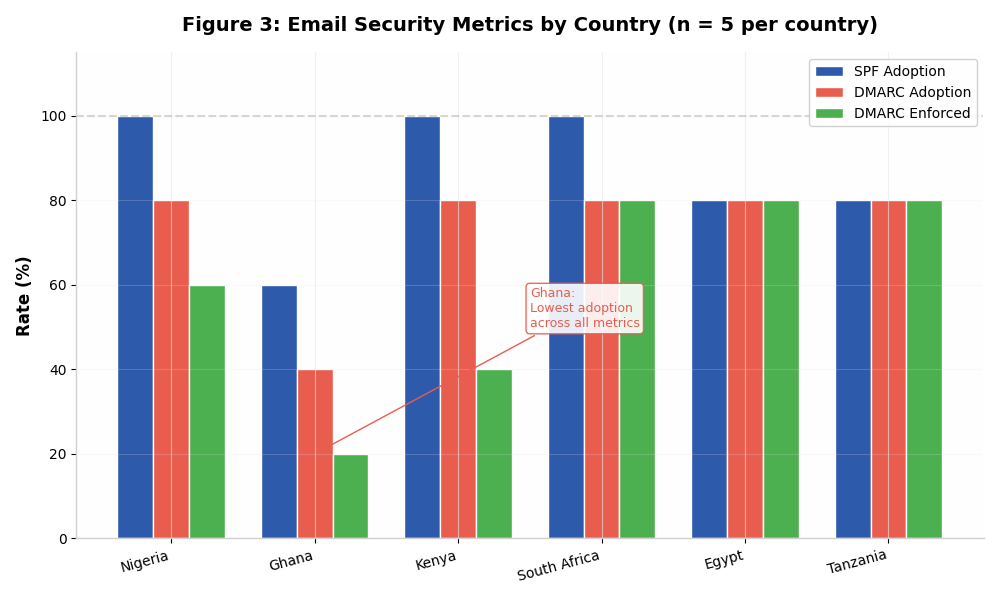
\includegraphics[width=\linewidth]{figure3_country_comparison.png}
    \caption{Email security metrics across 15 African nations ($n = 5$ organizations per country, $N=75$ total).}
    \label{fig:country}
\end{figure}

\subsection{Attack Surface Visibility (RQ1)}

Subdomain brute-forcing across the expanded 75-organization study revealed a mean of 13.24 resolvable hostnames per organization (SD = 33.29, range: 0--280) and 14.65 discovered public IP addresses (SD = 13.35, range: 0--56). The substantially increased upper bounds (Uganda at 65.8 mean subdomains, compared to the pilot maximum of 32.8) reflect the geographic diversity of the expanded sample, which captures institutions with larger, more complex infrastructure across multiple regional contexts. Figure~\ref{fig:attack_surface} shows the distribution by sector.

\begin{figure}[htbp]
    \centering
    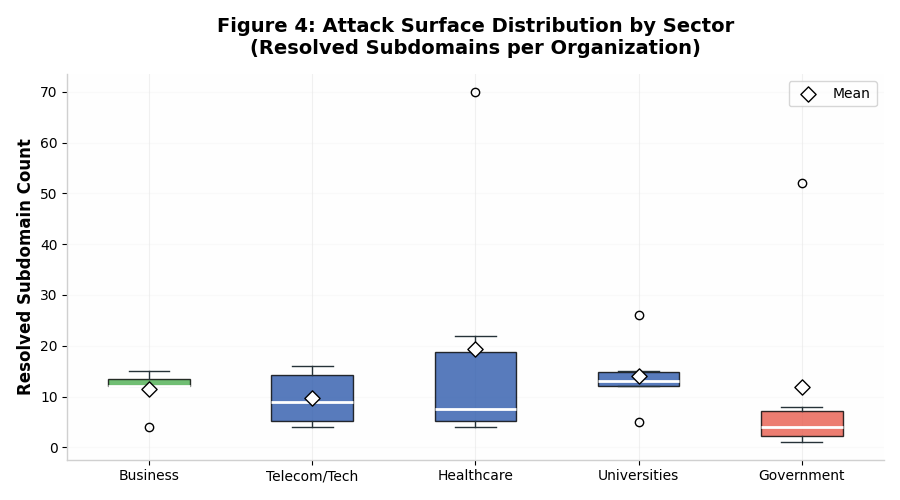
\includegraphics[width=\linewidth]{figure4_attack_surface.png}
    \caption{Attack surface distribution by sector: resolved subdomains per organization (N=75).}
    \label{fig:attack_surface}
\end{figure}

\subsection{Upstream Data Source Degradation (RQ5)}

A pivotal methodological finding concerns Certificate Transparency API reliability. Across the expanded 75-organization collection, approximately 96.7\% of CT collection requests encountered HTTP 504/502 timeouts or rate limits, necessitating fallback to root domain discovery only ($certificate\_domain\_count = 1$). Beacon addresses this by explicitly setting $certificate\_data\_available = \text{False}$ and $observed\_asset\_coverage = \text{null}$ when fallback occurs, preventing spurious coverage calculations. Multi-resolver validation across Google (8.8.8.8), Cloudflare (1.1.1.1), and Quad9 (9.9.9.9) DNS confirmed 100\% agreement on surviving targets, validating that measurement inconsistencies originate in third-party CT aggregators rather than target infrastructure changes.

\section{Discussion}

\subsection{The Adoption-Enforcement Gap}
While headline SPF adoption is high (86.7\%), over half of adopting domains (53.8\%) employ softfail mechanisms ($\sim$all or ?all). In modern mail processing, softfail instructs receiving MTAs to accept non-conforming messages with only spam scoring increments. Without strict DMARC alignment, attackers can forge sender addresses with minimal friction.

\subsection{The Government Exposure Paradox}
Our finding that 0.0\% of sampled government portals enforce DMARC---compared to 100\% of commercial banks---underscores a critical public-sector cyber hygiene challenge. Government domains are prime targets for state-sponsored phishing, tax scams, and executive impersonation. Implementing $p=\text{quarantine}$ and $p=\text{reject}$ policies on apex government domains represents an immediate, cost-effective defense.

\subsection{Measurement Implications}
The crt.sh degradation finding has broader implications for passive measurement research. Studies relying on public CT APIs without explicit availability flags risk severe coverage bias. We recommend that all passive measurement frameworks incorporate upstream source provenance tracking.

\section{Conclusion}

Beacon provides an open-source, reproducible, and ethically bounded framework for measuring observable organizational Internet exposure. The Africa pilot demonstrates that while core commercial and academic sectors have achieved high rates of email authentication adoption, severe structural vulnerabilities persist in public-sector apex domains. Future work will scale to 54 African economies, incorporate DNS-over-HTTPS multi-vantage collectors, and deploy automated longitudinal tracking.

\section*{Reproducibility Statement}

All dataset files, analysis scripts, and the measurement framework are released for independent replication. The anonymized dataset, statistical analysis engine, and validation tools are available at: \url{https://github.com/Rayxworld/Beacon}.

\begin{thebibliography}{10}

\bibitem{durumeric2014internet}
Z.~Durumeric et al., ``The Internet is Not a Big Truck,'' in \textit{Proc. IEEE S\&P}, 2014.

\bibitem{durumeric2013zmap}
Z.~Durumeric, E.~Wustrow, and J.~A. Halderman, ``ZMap: Fast Internet-wide Scanning and Its Security Applications,'' in \textit{Proc. USENIX Security}, 2013.

\bibitem{durumeric2015search}
Z.~Durumeric et al., ``An Internet-Wide View of Internet-Wide Scanning,'' in \textit{Proc. USENIX Security}, 2015.

\bibitem{matherly2015shodan}
J.~Matherly, ``Shodan: The Search Engine for the Internet of Things,'' 2015.

\bibitem{weimer2005passive}
F.~Weimer, ``Passive DNS Replication,'' in \textit{Proc. FIRST Conference}, 2005.

\bibitem{rfc6962}
B.~Laurie, A.~Langley, and E.~Kasper, ``Certificate Transparency,'' RFC 6962, 2013.

\bibitem{thomas2016transparency}
K.~Thomas et al., ``The Underground Economy of Certificate Transparency,'' in \textit{Proc. NDSS}, 2016.

\bibitem{rfc7208}
S.~Kitterman, ``Sender Policy Framework (SPF) for Authorizing Use of Domains in Email,'' RFC 7208, 2014.

\bibitem{rfc7489}
P.~Kucherawy and E.~Zwicky, ``Domain-based Message Authentication, Reporting, and Conformance (DMARC),'' RFC 7489, 2015.

\bibitem{fiebig2018}
T.~Fiebig et al., ``A Look at the Email Ecosystem Through the Lens of DMARC,'' in \textit{Proc. ACM IMC}, 2018.

\bibitem{klensin2019}
J.~Klensin, ``Email Authentication for Internationalized Email,'' \textit{Internet-Draft}, 2019.

\bibitem{moyo2020africa}
T.~Moyo and M.~Mutula, ``Cybersecurity Policy Frameworks in Africa,'' \textit{Journal of Information Security}, 2020.

\bibitem{ouedraogo2021threats}
A.~Ouedraogo et al., ``Cyber Threats in African Digital Infrastructure,'' in \textit{Proc. AFRICOMM}, 2021.

\bibitem{wilson1927probable}
E.~B. Wilson, ``Probable Inference, the Law of Succession, and Statistical Inference,'' \textit{Journal of the American Statistical Association}, 1927.

\bibitem{levchenko2016understanding}
K.~Levchenko et al., ``Understanding the Mirai Botnet,'' in \textit{Proc. USENIX Security}, 2016.

\bibitem{syverson2018certified}
P.~Syverson, ``Certified Phishing: Taking a Look at Certificate Transparency in Practice,'' in \textit{Proc. ACSAC}, 2018.

\end{thebibliography}

\end{document}
